\documentclass[a4paper,11pt]{article}

\usepackage[english]{babel} 
\usepackage[utf8]{inputenc}
\usepackage[cyr]{aeguill}
\usepackage{stmaryrd}

\usepackage{lmodern} %Type1-font for non-english texts and characters
\usepackage{caption}
\usepackage{subcaption}

\usepackage{graphicx}
\usepackage{hyperref}
\usepackage{listings}

\usepackage{epstopdf}

%% Math Packages 
\usepackage{amsmath}
\usepackage{amsthm}
\usepackage{amsfonts}
\usepackage{amssymb}
\usepackage{mathrsfs}
\usepackage{pst-all}
\usepackage{lscape}
\usepackage{pdfpages}
\usepackage{mathabx}


\usepackage{color, colortbl}
\definecolor{lightgray}{gray}{0.85}
\usepackage{multirow}
\usepackage[Algorithme]{algorithm}
\usepackage[noend]{algpseudocode}
\usepackage{tikz}

%\renewcommand{\algorithmicdo}{\textbf{faire}}
%\renewcommand{\algorithmicwhile}{\textbf{tant que}}


\usepackage{a4wide} %%Smaller margins = more text per page.
\usepackage{fancyhdr} %%Fancy headings

\setcounter{secnumdepth}{5}
\setcounter{tocdepth}{5}


\DeclareMathOperator*{\argmax}{arg\,max}
\DeclareMathOperator*{\argmin}{arg\,min}
\graphicspath{{/Users/melisandezonta/Documents/Documents/Documents/GTL_courses_second_semester/Computer-Vision/PS5-all/PS5-input/}}




\usepackage{listings}
\usepackage{color}
 
\definecolor{codegreen}{rgb}{0,0.6,0}
\definecolor{codegray}{rgb}{0.5,0.5,0.5}
\definecolor{codepurple}{rgb}{0.58,0,0.82}
\definecolor{backcolour}{rgb}{0.95,0.95,0.92}
 
\lstdefinestyle{mystyle}{
    backgroundcolor=\color{backcolour},   
    commentstyle=\color{codegreen},
    keywordstyle=\color{magenta},
    numberstyle=\tiny\color{codegray},
    stringstyle=\color{codepurple},
    basicstyle=\footnotesize,
    breakatwhitespace=false,         
    breaklines=true,                 
    captionpos=b,                    
    keepspaces=true,                 
    numbers=left,                    
    numbersep=5pt,                  
    showspaces=false,                
    showstringspaces=false,
    showtabs=false,                  
    tabsize=2
}
 
\lstset{style=mystyle}

\begin{document}

%\pagestyle{fancy}

\begin{titlepage}
\vspace*{\stretch{1}}

\begin{center}

\includegraphics[scale=0.4]{GT_logo.jpeg}
\end{center}
\vspace*{\stretch{1}}
\hrulefill
\begin{center}\bfseries\huge
   Computer Vision \\
   CS 6476 , Spring 2018\\
   \end{center}
  \begin{center}\bfseries\large
     PS 5\\
    \hrulefill
\end{center}
%\hfill
\vspace*{1cm}
\begin{minipage}[t]{0.6\textwidth}
  \begin{flushleft} \large
    \emph{Professor : }\\
    Cedric Pradalier \\
  \end{flushleft}
\end{minipage}
\begin{minipage}[t]{0.3\textwidth}
  \begin{flushright} \large
    \emph{Author :} \\
    Melisande Zonta \\
  \end{flushright}
\end{minipage}
\vspace*{\stretch{2}}
\begin{flushright}
       \today 
\end{flushright} 
\end{titlepage}

\tableofcontents
\clearpage




\section{Gaussian and Laplacian Pyramids}

\subsection{Reduce}

We start by implementing the reduce operator using the function below, which allows us to compute the Gaussian pyramid.

A first step of preprocessing was executed by creating a function to apply zero padding if the size of the image is not of a power of 2.
 
Then another function allows us to cut the resulting image in order to remove the zero padding. Finally the borders were taken in charge by using the built-in OpenCV function \textit{copyMakeBorder} with the replication option.

\lstset{style=mystyle}
\lstinputlisting[language=Python, firstline=24, lastline=42]{/Users/melisandezonta/Documents/Documents/Documents/GTL_courses_second_semester/Computer-Vision/PS5-all/PS5-code/Functions.py}

\lstset{style=mystyle}
\lstinputlisting[language=Python, firstline=44, lastline=60]{/Users/melisandezonta/Documents/Documents/Documents/GTL_courses_second_semester/Computer-Vision/PS5-all/PS5-code/Functions.py}


 \begin{figure}[H]
\begin{center}
\begin{tabular}{c}
	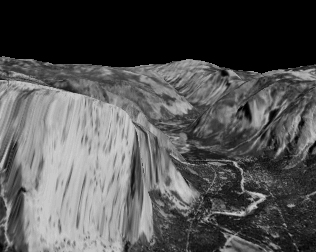
\includegraphics{ps5-1-1-0.png}\\
	a\\
	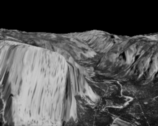
\includegraphics{ps5-1-1-1.png}\\
	b\\
	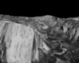
\includegraphics{ps5-1-1-2.png}\\
	c\\
	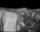
\includegraphics{ps5-1-1-3.png}\\
	d
\end{tabular}
\end{center}
\caption{ 
\textit{a}. ps5-1-1-0.png.  \textit{b}. ps5-1-1-0.png. \textit{c}. ps5-1-1-2.png.  \textit{d}. ps5-1-1-3.png.  }
\label{ps-5-1}
\end{figure}

The images presented in Figure \ref{ps-5-1} a, b, c and d show the levels 0 to 3 of the Gaussian pyramid for the first frame of DataSeq1.



\subsection{Expand}

Now we write the expand function, that will allow us to build the hierarchical Lucas-Kanade akgorithm.
We test it here by computing the Laplacian pyramid from the Gaussian pyramid of DataSeq1.

\lstset{style=mystyle}
\lstinputlisting[language=Python, firstline=64, lastline=86]{/Users/melisandezonta/Documents/Documents/Documents/GTL_courses_second_semester/Computer-Vision/PS5-all/PS5-code/Functions.py}

\begin{figure}[H]
\begin{center}
\begin{tabular}{c}
	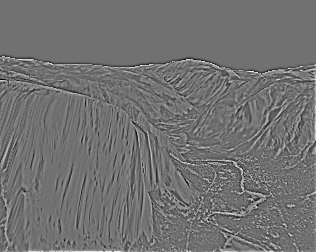
\includegraphics{ps5-1-2-0.png}\\
	a\\
	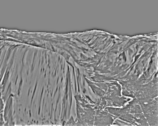
\includegraphics{ps5-1-2-1.png}\\
	b\\
	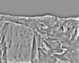
\includegraphics{ps5-1-2-2.png}\\
	c\\
	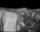
\includegraphics{ps5-1-2-3.png}\\
	d
\end{tabular}
\end{center}
\caption{ 
\textit{a}. ps5-1-2-0.png.  \textit{b}. ps5-1-2-1.png. \textit{c}. ps5-1-2-2.png.  \textit{d}. ps5-1-2-3.png.  }
\label{ps-5-2}
\end{figure}


The resulting images (Figure \ref{ps-5-2} a, b, c and d)  show the Laplacian pyramid level 0 to level 3 (the last level of the Gaussian pyramid).

\section{Lucas-Kanade Optic Flow}

\subsection{Lucas-Kanade for Small Displacements}

The next step is to implement the Lucas-Kanade computation. 
We first prefer to smooth the images and using a Gaussian kernel convolution.
In order to remove outliers that are breaking the smooth motion assumption, a median filter is applied to the resulting displacement images.
The parameters used for the following tests were a window size of 20 pixels and a sigma of 5.

\lstset{style=mystyle}
\lstinputlisting[language=Python, firstline=91, lastline=138]{/Users/melisandezonta/Documents/Documents/Documents/GTL_courses_second_semester/Computer-Vision/PS5-all/PS5-code/Functions.py}



\begin{figure}[H]
\begin{center}
\begin{tabular}{cc}
	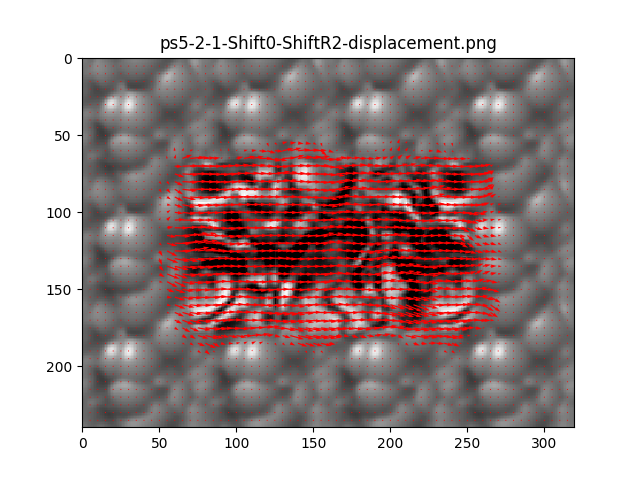
\includegraphics[width=.5 \textwidth]{ps5-2-1-Shift0-ShiftR2-displacement.png}&
	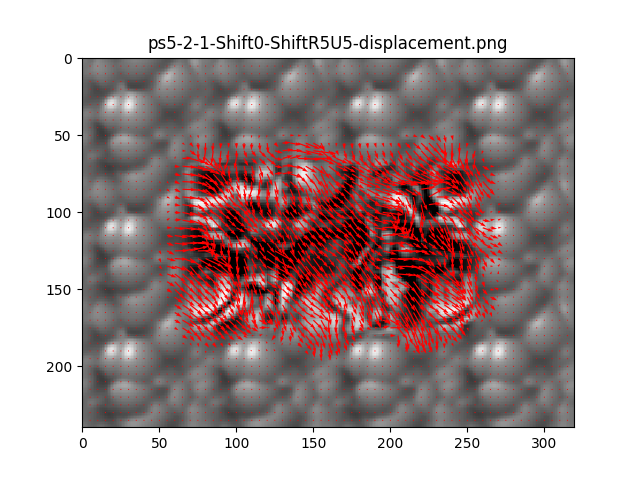
\includegraphics[width=.5 \textwidth]{ps5-2-1-Shift0-ShiftR5U5-displacement.png}\\
	a&b
\end{tabular}
\end{center}
\caption{ 
\textit{a}.ps5-2-1-Shift0-ShiftR2-displacement.png.  \textit{b}.ps5-2-1-Shift0-ShiftR5U5-displacement.png.  }
\label{ps-5-3}
\end{figure}

We test the process upon the textured images, the first one shifted by 2 pixels to the right (result in Figure \ref{ps-5-3} a) and the second one shifted by 5 pixels right and up (Figure \ref{ps-5-3} b).

\subsection{Lucas-Kanade for Larger Displacements}

We now try to apply the same algorithm, using the same parameters, to images with larger motions (10, 20 and 40 pixels).

\begin{figure}[H]
\begin{center}
\begin{tabular}{cc}
	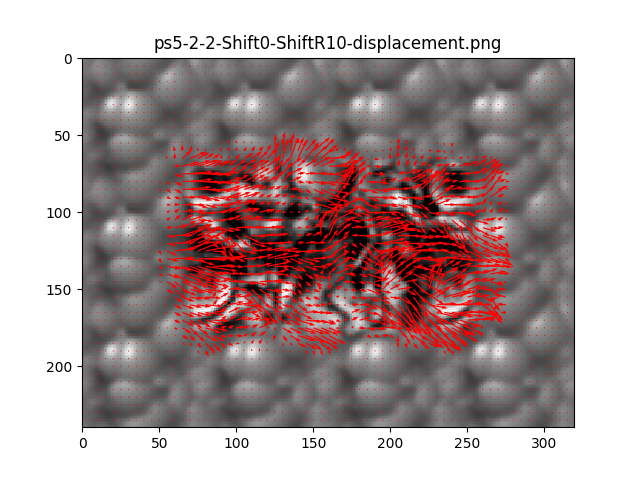
\includegraphics[width=.5 \textwidth]{ps5-2-2-Shift0-ShiftR10-displacement.png}&
	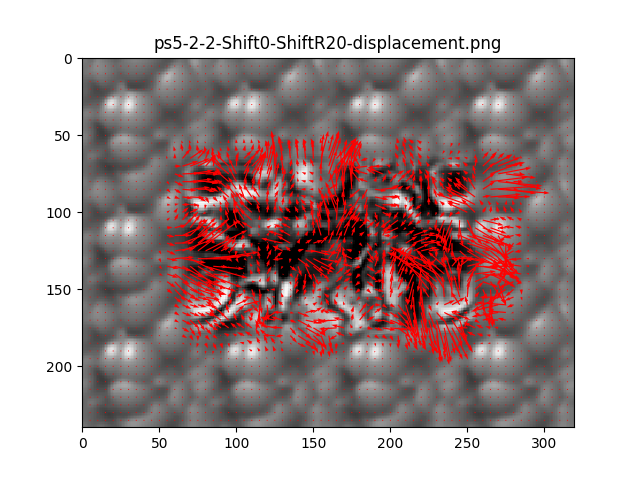
\includegraphics[width=.5 \textwidth]{ps5-2-2-Shift0-ShiftR20-displacement.png}\\
	a&b\\
	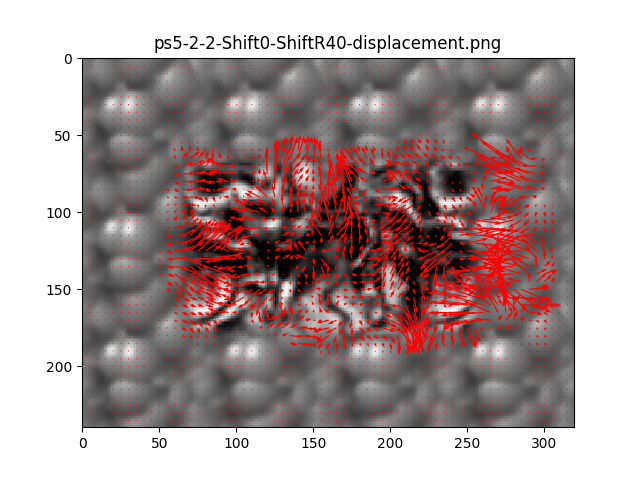
\includegraphics[width=.5 \textwidth]{ps5-2-2-Shift0-ShiftR40-displacement.png}\\
	c
\end{tabular}
\end{center}
\caption{ 
\textit{a}. ps5-2-2-Shift0-ShiftR10-displacement.png.  \textit{b}. ps5-2-2-Shift0-ShiftR20-displacement.png. \textit{c}. ps5-2-2-Shift0-ShiftR40-displacement.png.  }
\label{ps-5-4}
\end{figure}

The respective results are visible in Figure \ref{ps-5-4} a,b and c.
We notice that although some kind of consistency in the displacement amplitude is visible for a shift of 10 pixels, the orientation is definitely wrong. For higher shifts, the resulting displacements are completely wrong.
This is explained by the fact that the Lucas-Kanade algorithm, used at a fine level of the pyramid (here the full resolution image), works only for small motions (a few pixels), since it assumes a local consistency of motion.

\subsection{Lucas-Kanade applied on more realistic images}

We now try our algorithm on more realistic images (DataSeq1 and DataSeq2). 
We continue to use a single-level version of Lucas-Kanade, but allow ourselves to choose the level in the Gaussian pyramid that seems to work best.
We then warp the first image to the second, using the recovered displacement images with the following code : 
\lstset{style=mystyle}
\lstinputlisting[language=Python, firstline=139, lastline=148]{/Users/melisandezonta/Documents/Documents/Documents/GTL_courses_second_semester/Computer-Vision/PS5-all/PS5-code/Functions.py}


\begin{figure}[H]
\begin{center}
\begin{tabular}{cc}
	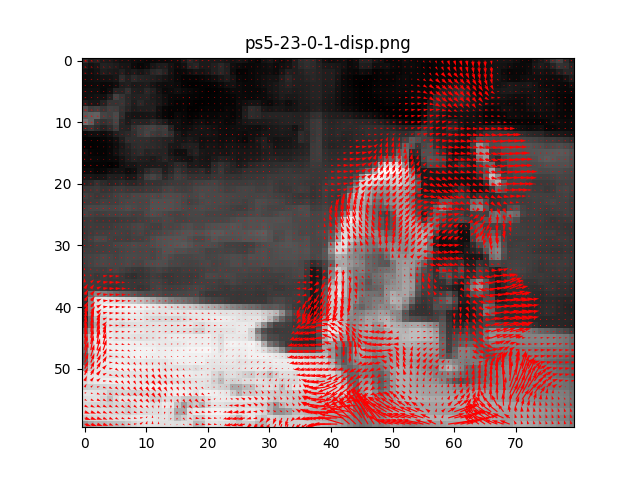
\includegraphics[width=.5 \textwidth]{ps5-2-3-0-1-displacement.png}&
	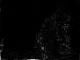
\includegraphics[width=.5 \textwidth]{ps5-2-3-0-1-diff.png}\\
	a&b\\
	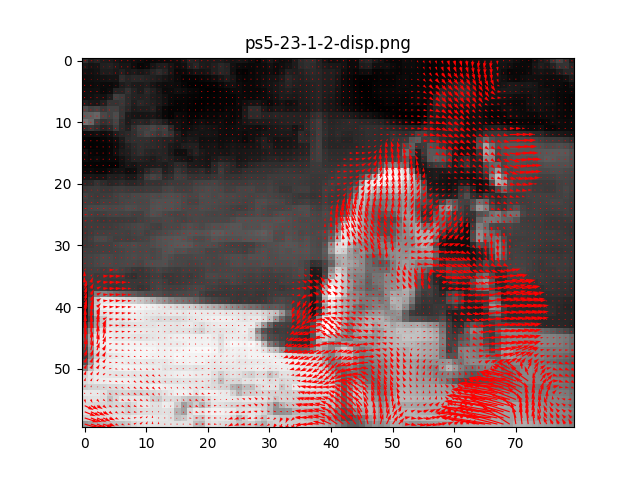
\includegraphics[width=.5 \textwidth]{ps5-2-3-1-2-displacement.png}&
	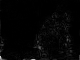
\includegraphics[width=.5 \textwidth]{ps5-2-3-1-2-diff.png}\\
	c&d
\end{tabular}
\end{center}
\caption{ 
\textit{a}. ps5-2-3-0-1-displacement.png.  \textit{b}. ps5-2-3-0-1-diff.png. \textit{c}. ps5-2-3-1-2-displacement.png.  \textit{d}. ps5-2-3-1-2-diff.png. }
\label{ps-5-5-a}
\end{figure}



\begin{figure}[H]
\begin{center}
\begin{tabular}{cc}
	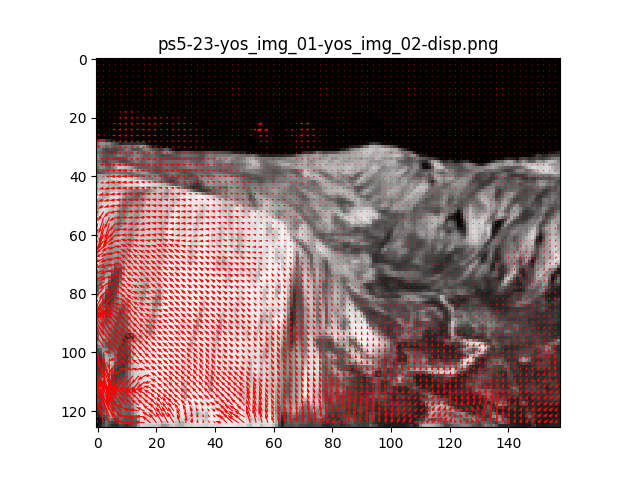
\includegraphics[width=.5 \textwidth]{ps5-2-3-yos_img_01-yos_img_02-displacement.png}&
	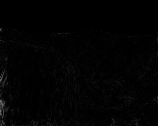
\includegraphics[width=.5 \textwidth]{ps5-2-3-yos_img_01-yos_img_02-diff.png}\\
	a&b\\
	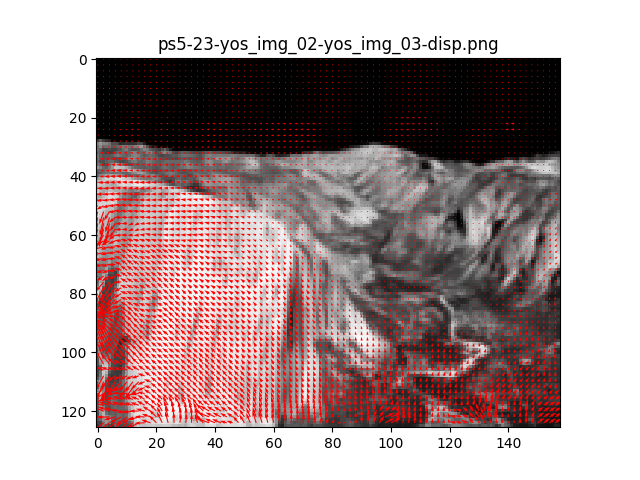
\includegraphics[width=.5 \textwidth]{ps5-2-3-yos_img_02-yos_img_03-displacement.png}&
	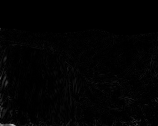
\includegraphics[width=.5 \textwidth]{ps5-2-3-yos_img_02-yos_img_03-diff.png}\\
	c&d
\end{tabular}
\end{center}
\caption{ 
\textit{a}. ps5-2-3-yos-img-01-yos-img-02-displacement.png.  \textit{b}. ps5-2-3-yos-img-01-yos-img-02-diff.png. \textit{c}. ps5-2-3-yos-img-02-yos-img-03-displacement.png.  \textit{d} ps5-2-3-yos-img-02-yos-img-03-diff.png. }
\label{ps-5-5-b}
\end{figure}


Concerning DataSeq2, the level selected was the third level in the pyramid. \\
The figures \ref{ps-5-5-a}a and b show the difference and displacement images when warping the first frame to the second one.\\
The figures \ref{ps-5-5-a}c and d show the difference and displacement images when warping the second frame to the third one.\\

Then we study DataSeq1 and we observe that the best results are obtained for the second level of the pyramid.\\
The figures \ref{ps-5-5-b}a and b show the difference and displacement images when warping the first frame to the second one.\\
The figures \ref{ps-5-5-b}c and d show the difference and displacement images when warping the second frame to the third one.\\

We can state several problems and observations on the previous images : 
\begin{itemize}
\item There is a problem on the edges of the images, which could be explained by a wrong handling of the borders of the images.
\item The computations seems to work best for DataSeq1 than for DataSeq2 which could be explain by smaller motions spread on the entire image whereas the motions are stronger and more localized in some regions of the image. That's why a coarser level was used for DataSeq2 with a smaller window.
\end{itemize}

\section{Hierarchical Lucas-Kanade}

Now we are going to implement a multi-level of the Lucas-Kanade algorithm that is using Gaussian Pyramids, the warping and expand functions so we can initialize the next level with the previous level displacement image.

\lstset{style=mystyle}
\lstinputlisting[language=Python, firstline=151, lastline=190]{/Users/melisandezonta/Documents/Documents/Documents/GTL_courses_second_semester/Computer-Vision/PS5-all/PS5-code/Functions.py}

Then we apply successively this algorithm on the TestSeq, DataSeq1 and DataSeq2.



\begin{figure}[H]
\begin{center}
\begin{tabular}{cc}
	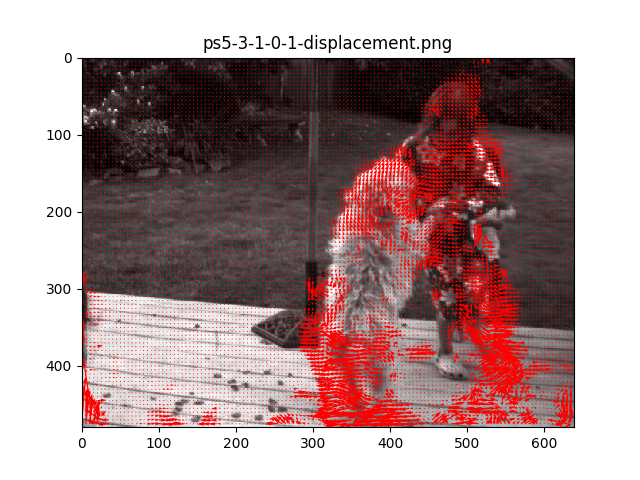
\includegraphics[width=.5 \textwidth]{ps5-3-1-0-1-displacement.png}&
	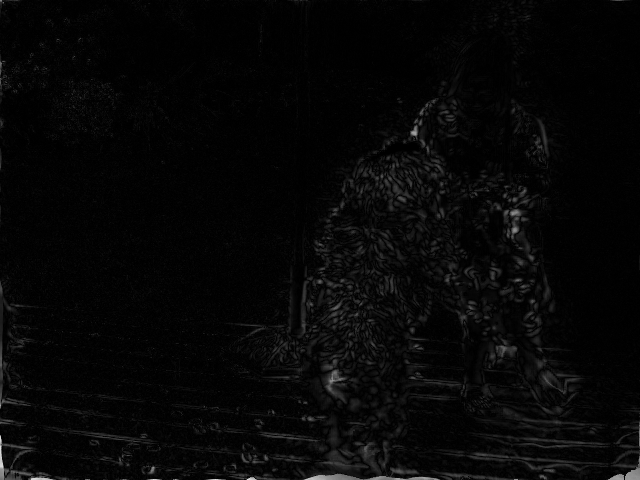
\includegraphics[width=.5 \textwidth]{ps5-3-1-0-1-diff.png}\\
	a&b\\
	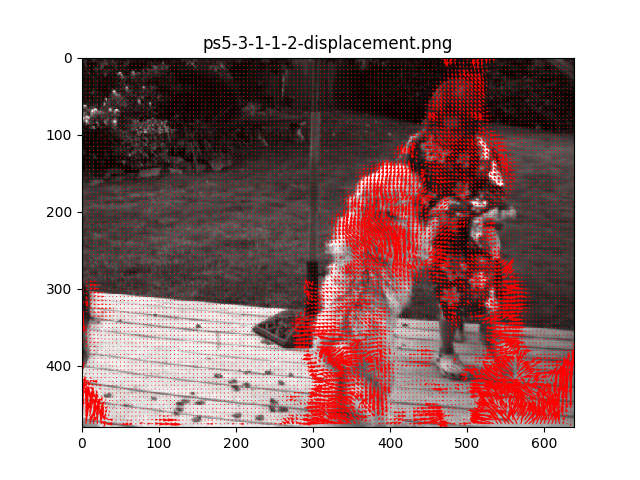
\includegraphics[width=.5 \textwidth]{ps5-3-1-1-2-displacement.png}&
	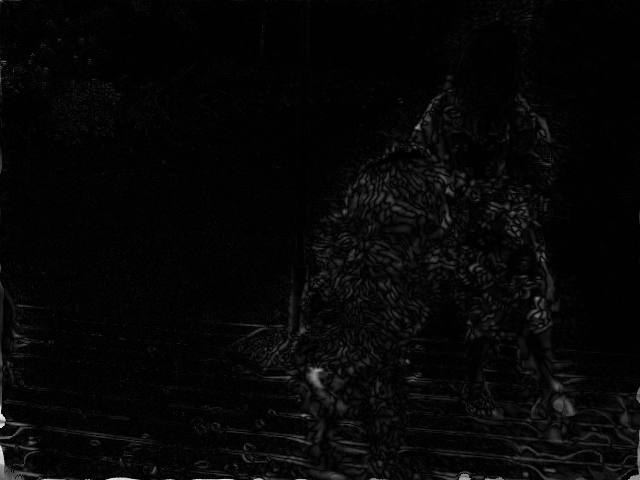
\includegraphics[width=.5 \textwidth]{ps5-3-1-1-2-diff.png}\\
	c&d
\end{tabular}
\end{center}
\caption{ 
\textit{a}. ps5-3-1-0-1-displacement.png.  \textit{b}. ps5-3-1-0-1-diff.png. \textit{c}. ps5-3-1-1-2-displacement.png.  \textit{d}. ps5-3-1-1-2-diff.png. }
\label{ps-5-6-a}
\end{figure}



\begin{figure}[H]
\begin{center}
\begin{tabular}{cc}
	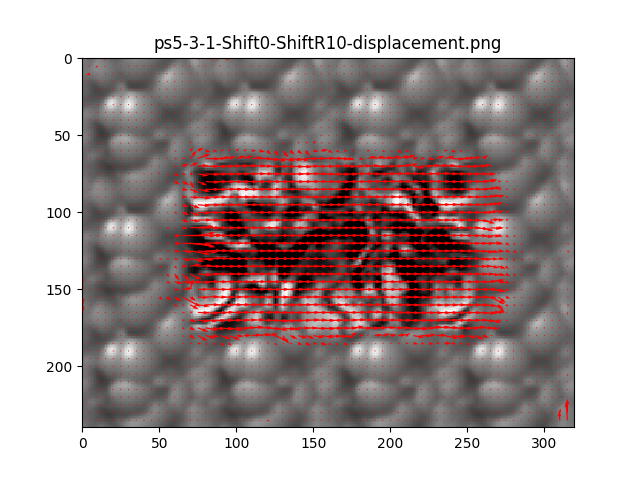
\includegraphics[width=.5 \textwidth]{ps5-3-1-Shift0-ShiftR10-displacement.png}&
	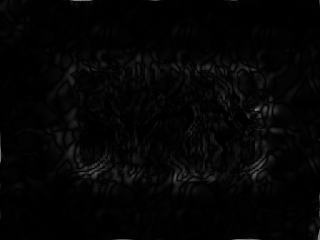
\includegraphics[width=.5 \textwidth]{ps5-3-1-Shift0-ShiftR10-diff.png}\\
	e&f\\
	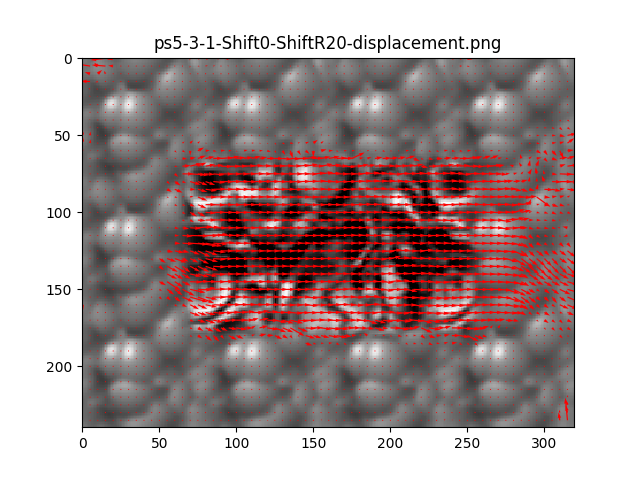
\includegraphics[width=.5 \textwidth]{ps5-3-1-Shift0-ShiftR20-displacement.png}&
	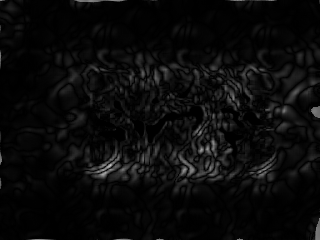
\includegraphics[width=.5 \textwidth]{ps5-3-1-Shift0-ShiftR20-diff.png}\\
	g&h\\
	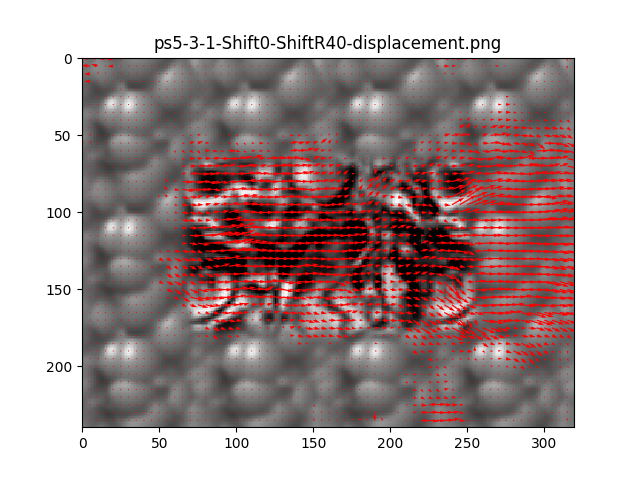
\includegraphics[width=.5 \textwidth]{ps5-3-1-Shift0-ShiftR40-displacement.png}&
	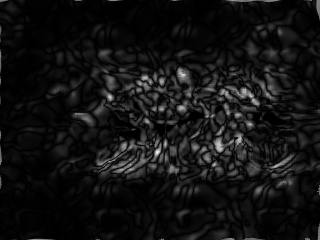
\includegraphics[width=.5 \textwidth]{ps5-3-1-Shift0-ShiftR40-diff.png}\\
	g&h
\end{tabular}
\end{center}
\caption{ 
\textit{a}. ps5-3-1-Shift0-ShiftR10-displacement.png.  \textit{b}. ps5-3-1-Shift0-ShiftR10-diff.png. \textit{c}. ps5-3-1-Shift0-ShiftR20-displacement.png.  \textit{d} ps5-3-1-Shift0-ShiftR20-diff.png.  \textit{e} ps5-3-1-Shift0-ShiftR40-displacement.png \textit{f} ps5-3-1-Shift0-ShiftR40-diff.png}
\label{ps-5-6-b}
\end{figure}


\begin{figure}[H]
\begin{center}
\begin{tabular}{cc}
	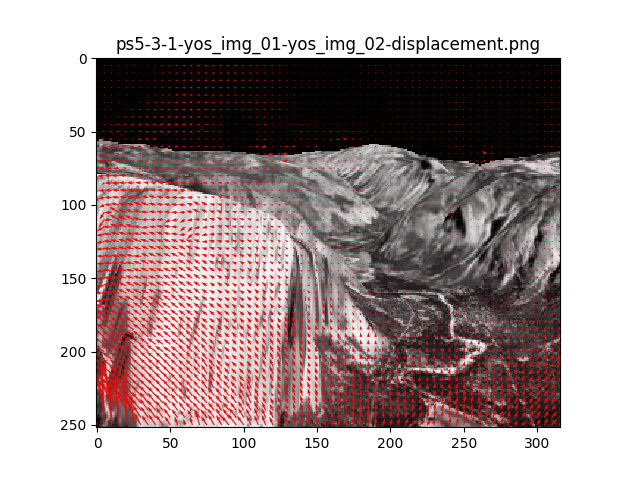
\includegraphics[width=.5 \textwidth]{ps5-3-1-yos_img_01-yos_img_02-displacement.png}&
	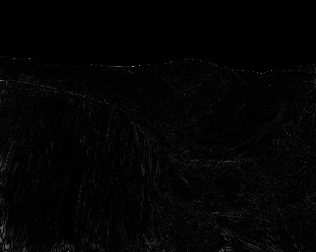
\includegraphics[width=.5 \textwidth]{ps5-3-1-yos_img_01-yos_img_02-diff.png}\\
	a&b\\
	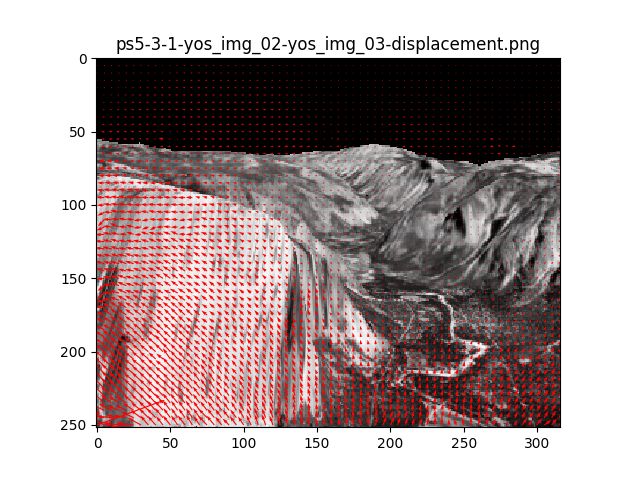
\includegraphics[width=.5 \textwidth]{ps5-3-1-yos_img_02-yos_img_03-displacement.png}&
	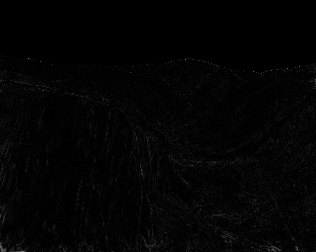
\includegraphics[width=.5 \textwidth]{ps5-3-1-yos_img_02-yos_img_03-diff.png}\\
	c&d
\end{tabular}
\end{center}
\caption{ 
\textit{a}. ps5-3-1-yos-img-01-yos-img-02-displacement.png.  \textit{b}. ps5-3-1-yos-img-01-yos-img-02-diff.png. \textit{c}. ps5-3-1-yos-img-02-yos-img-03-displacement.png.  \textit{d}. ps5-3-1-yos-img-02-yos-img-03-diff.png. }
\label{ps-5-6-c}
\end{figure}

We observe again several things in the previous results : 
\begin{itemize}
\item We obtain better result for the TestSeq 10 and 20 pixels shifts than with a single-level LK.
\item The process works also fine for DataSeq1 images but the results are not as good for DataSeq2 still because of the strong boundaries issues.
\item For coarser levels, adding a large smoothing and weighting window will result in a very important averaging that might not be the best solution especially for very localized motions as in DataSeq2
\end{itemize}


\section{The Juggle Sequence}

Finally we test our Hierarchical Luka Kanade on frames of a juggler and we try to detect the motion of his arms and juggling balls.\\
But as for DataSeq2, the motions are very localized and quite larger so we expect our implementation not to perform well.

\begin{figure}[H]
\begin{center}
\begin{tabular}{cc}
	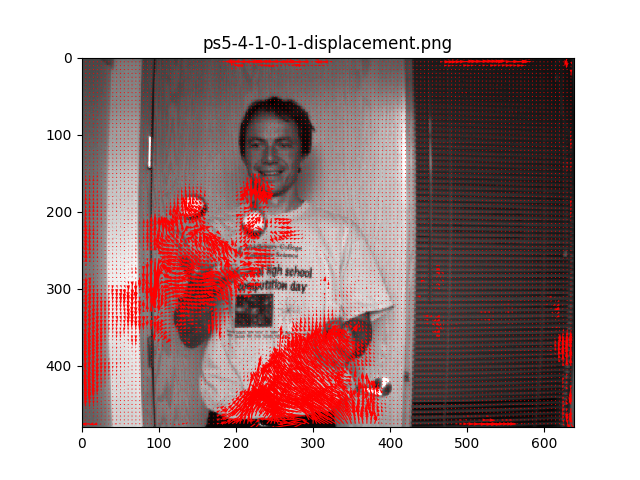
\includegraphics[width=.5 \textwidth]{ps5-4-1-0-1-displacement.png}&
	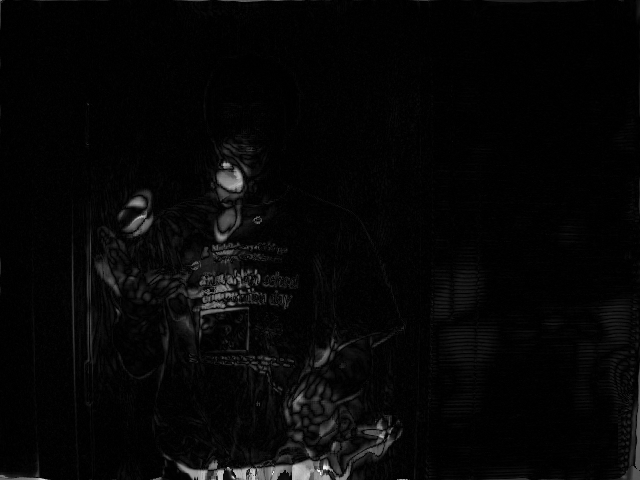
\includegraphics[width=.5 \textwidth]{ps5-4-1-0-1-diff.png}\\
	a&b\\
	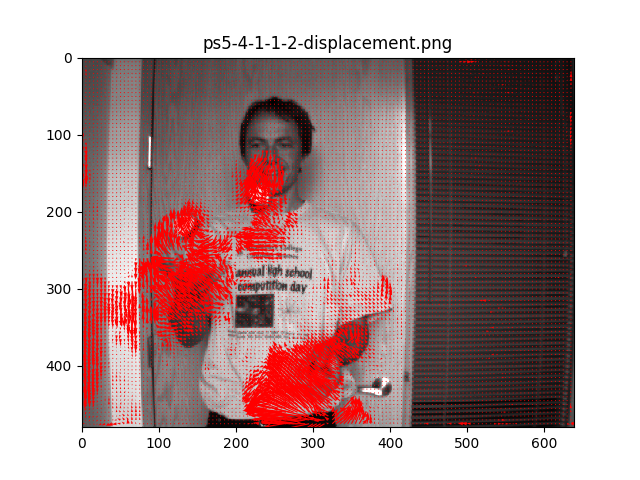
\includegraphics[width=.5 \textwidth]{ps5-4-1-1-2-displacement.png}&
	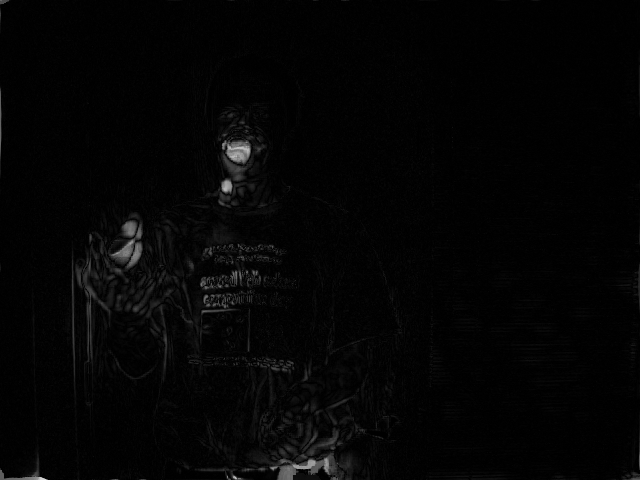
\includegraphics[width=.5 \textwidth]{ps5-4-1-1-2-diff.png}\\
	c&d
\end{tabular}
\end{center}
\caption{ 
\textit{a}. ps5-4-1-0-1-displacement.png.  \textit{b}. ps5-4-1-0-1-diff.png. \textit{c}. ps5-4-1-1-2-displacement.png.  \textit{d}. ps5-4-1-1-2-diff.png. }
\label{ps-5-7}
\end{figure}

\end{document}